
\documentclass[12pt]{article}
\usepackage{amsmath}
\usepackage{graphicx}
\usepackage{caption}
\usepackage{subcaption}
\usepackage{booktabs}
\usepackage{float}
\usepackage[utf8]{inputenc}
\usepackage[a4paper, margin=0.8in, bottom=0.7in]{geometry}

\usepackage{multirow}
\usepackage{setspace}
\usepackage{listings}
\usepackage{parskip}
\usepackage{svg}
\usepackage[bottom]{footmisc}
\usepackage{tikz}
\usepackage[title]{appendix}
\usepackage{biblatex}
\usepackage[section]{placeins}
\usepackage[newfloat]{minted}
\usepackage{lipsum}  
\usepackage{titlesec}


\addbibresource{mybiblio.bib} 
%\usepackage{pgfplots}
%\usepackage[caption=false]{subfig}

% This style is used to create block diagrams, you'll find it useful since many of your figures would be of that form, I'll try add more styles in the future :)
\usetikzlibrary{trees,positioning,fit,calc}
\tikzset{block/.style = {draw, fill=blue!20, rectangle,
                         minimum height=3em, minimum width=4em},
        input/.style = {coordinate},
        output/.style = {coordinate}
}

% Set space before and after sections
\titlespacing*{\section}{0pt}{*1}{*0.5}

% Set space before and after subsections
\titlespacing*{\subsection}{0pt}{*0.5}{*0.2}



\setlength{\textfloatsep}{3pt} % Adjust the space after a figure




\usepackage{minted}
\usepackage{xcolor}
\usemintedstyle{borland}

\counterwithin{figure}{section}
\counterwithin{table}{section}
\counterwithin{listing}{section}

\renewcommand{\arraystretch}{1.5}

\usepackage[hidelinks]{hyperref}
\hypersetup{
    linktoc=all
}

%\renewcommand\listingscaption{Listing}

\usepackage{tocbasic}
\setuptoc{lol}{levelup}

\setlength{\parindent}{0em}
\setlength{\parskip}{0em}


\definecolor{dkgreen}{rgb}{0,0.6,0}
\definecolor{gray}{rgb}{0.5,0.5,0.5}
\definecolor{mauve}{rgb}{0.58,0,0.82}

\lstset{frame=tb,
  language=HTML,
  aboveskip=3mm,
  belowskip=3mm,
  showstringspaces=false,
  columns=flexible,
  basicstyle={\small\ttfamily},
  numbers=none,
  numberstyle=\tiny\color{gray},
  keywordstyle=\color{blue},
  commentstyle=\color{dkgreen},
  stringstyle=\color{mauve},
  breaklines=true,
  breakatwhitespace=true,
  tabsize=3
}

%----------EDIT COVER INFO HERE -----------------%

\def \LOGOPATH {./assets/birzeit-logo.svg}
\def \FACULTY {Faculty of Engineering and Technology}
\def \DEPARTEMENT {Department of Electrical and Computer Engineering}
\def \COURSENUM {ENCS5341}
\def \COURSENAME {Machine Learning and Data Science}
\def \ASSIGNMENTTITLE {Assignment 3:}
\def \ASSIGNMENTDESCRIPTION {Machine Learning Algorithms Evaluation}
\def \STUDENTNAME {Karim Marayta}
\def \STUDENTID {1211610}
\def \STUDENTSEC {1}
\def \SECONDSTUDENTNAME {Mohammed Abed Alkareem}
\def \SECONDSTUDENTID {1210708}
\def \SECONDSTUDENTSEC {2}
\def \INSTRUCTOR {Dr. Yazan Abu Farha, Dr. Ismail Khater}
\def \ASSISTANT {dasf}

%------------------------------------------------%

\begin{document}

\pagenumbering{Roman}

\begin{titlepage}
    \vfill
    \begin{center}
        \includesvg[width=0.7\textwidth]{./assets/birzeit-logo.svg} 
        \hfill \\
        \Large{\FACULTY} \\
        \Large{\DEPARTEMENT} \\
        \vspace{0.5cm}
        \Large{\COURSENUM\textemdash\COURSENAME} \\
        \vfill
        \textbf{\LARGE{\ASSIGNMENTTITLE}} \\
        \textbf{\LARGE{\ASSIGNMENTDESCRIPTION}} \\
        \vspace{20pt}
        \Large{\textbf{Prepared by:\\} \STUDENTNAME\textemdash\STUDENTID\textemdash Section: \STUDENTSEC\\\SECONDSTUDENTNAME\textemdash\SECONDSTUDENTID\textemdash Section: \SECONDSTUDENTSEC}
    \end{center}
    \vfill
    \begin{flushleft}
        \Large{\textbf{Instructor:} \INSTRUCTOR} \\
%        \Large{\textbf{Assistant:} \ASSISTANT} \\
        \Large{\textbf{Date:} \today}
    \end{flushleft}
    \vspace{1in}
\end{titlepage}


%-----------------------------------------------%


\clearpage

\setlength{\parskip}{\baselineskip}%

\pagenumbering{arabic}


\section{Introduction}

The Breast Cancer dataset is widely used for binary classification tasks in machine learning. This dataset consists of features computed from digitized images of fine needle aspirate (FNA) of breast masses, aimed at classifying tumors as either malignant or benign. It contains a total of 569 samples with 30 real-valued features per sample, such as mean, standard error, and worst values of various geometric measures like radius, texture, perimeter, area, and smoothness.\cite{utkarsh2023breastcancer}



The dataset is particularly suitable for supervised learning methods and classification tasks due to its balanced class distribution:

\textbf{Malignant samples:} 212, \textbf{Benign samples:} 357


In this assignment, we utilize the Breast Cancer dataset to explore and evaluate machine learning models including K-Nearest Neighbors (KNN), Logistic Regression, Support Vector Machines (SVM), and ensemble methods like Boosting (AdaBoost) and Bagging (Random Forest). The primary objective is to compare the performance of these algorithms using key classification metrics, such as accuracy, precision, recall, F1-score, and ROC-AUC.

By experimenting with various configurations (e.g., different distance metrics in KNN, kernel types in SVM, and regularization techniques in Logistic Regression, different number of estimators in Random Forest and AdaBoost), this assignment aims to provide insights into the behavior and effectiveness of these models on real-world data.





\section{Dataset Exploration}


To understand the structure and characteristics of the Breast Cancer dataset, a thorough exploration was performed. The dataset contains 569 samples with 30 numerical features, which are derived from geometric properties of breast mass images. These features include measurements such as the mean, standard error, and worst values of radius, texture, perimeter, area, and smoothness.

The data was inspected to ensure its quality and reliability:
\begin{itemize}
    \item \textbf{Missing Values:} A check for missing or null values showed that the dataset is complete, with no missing entries.
    \item \textbf{Outliers:} Visual inspection using histograms and box plots indicated no significant outliers, as all feature values are well-behaved and lie within reasonable ranges.
\end{itemize}

\begin{figure}[h!]
    \centering
    % Histograms
    \begin{minipage}{0.49\textwidth}
        \centering
        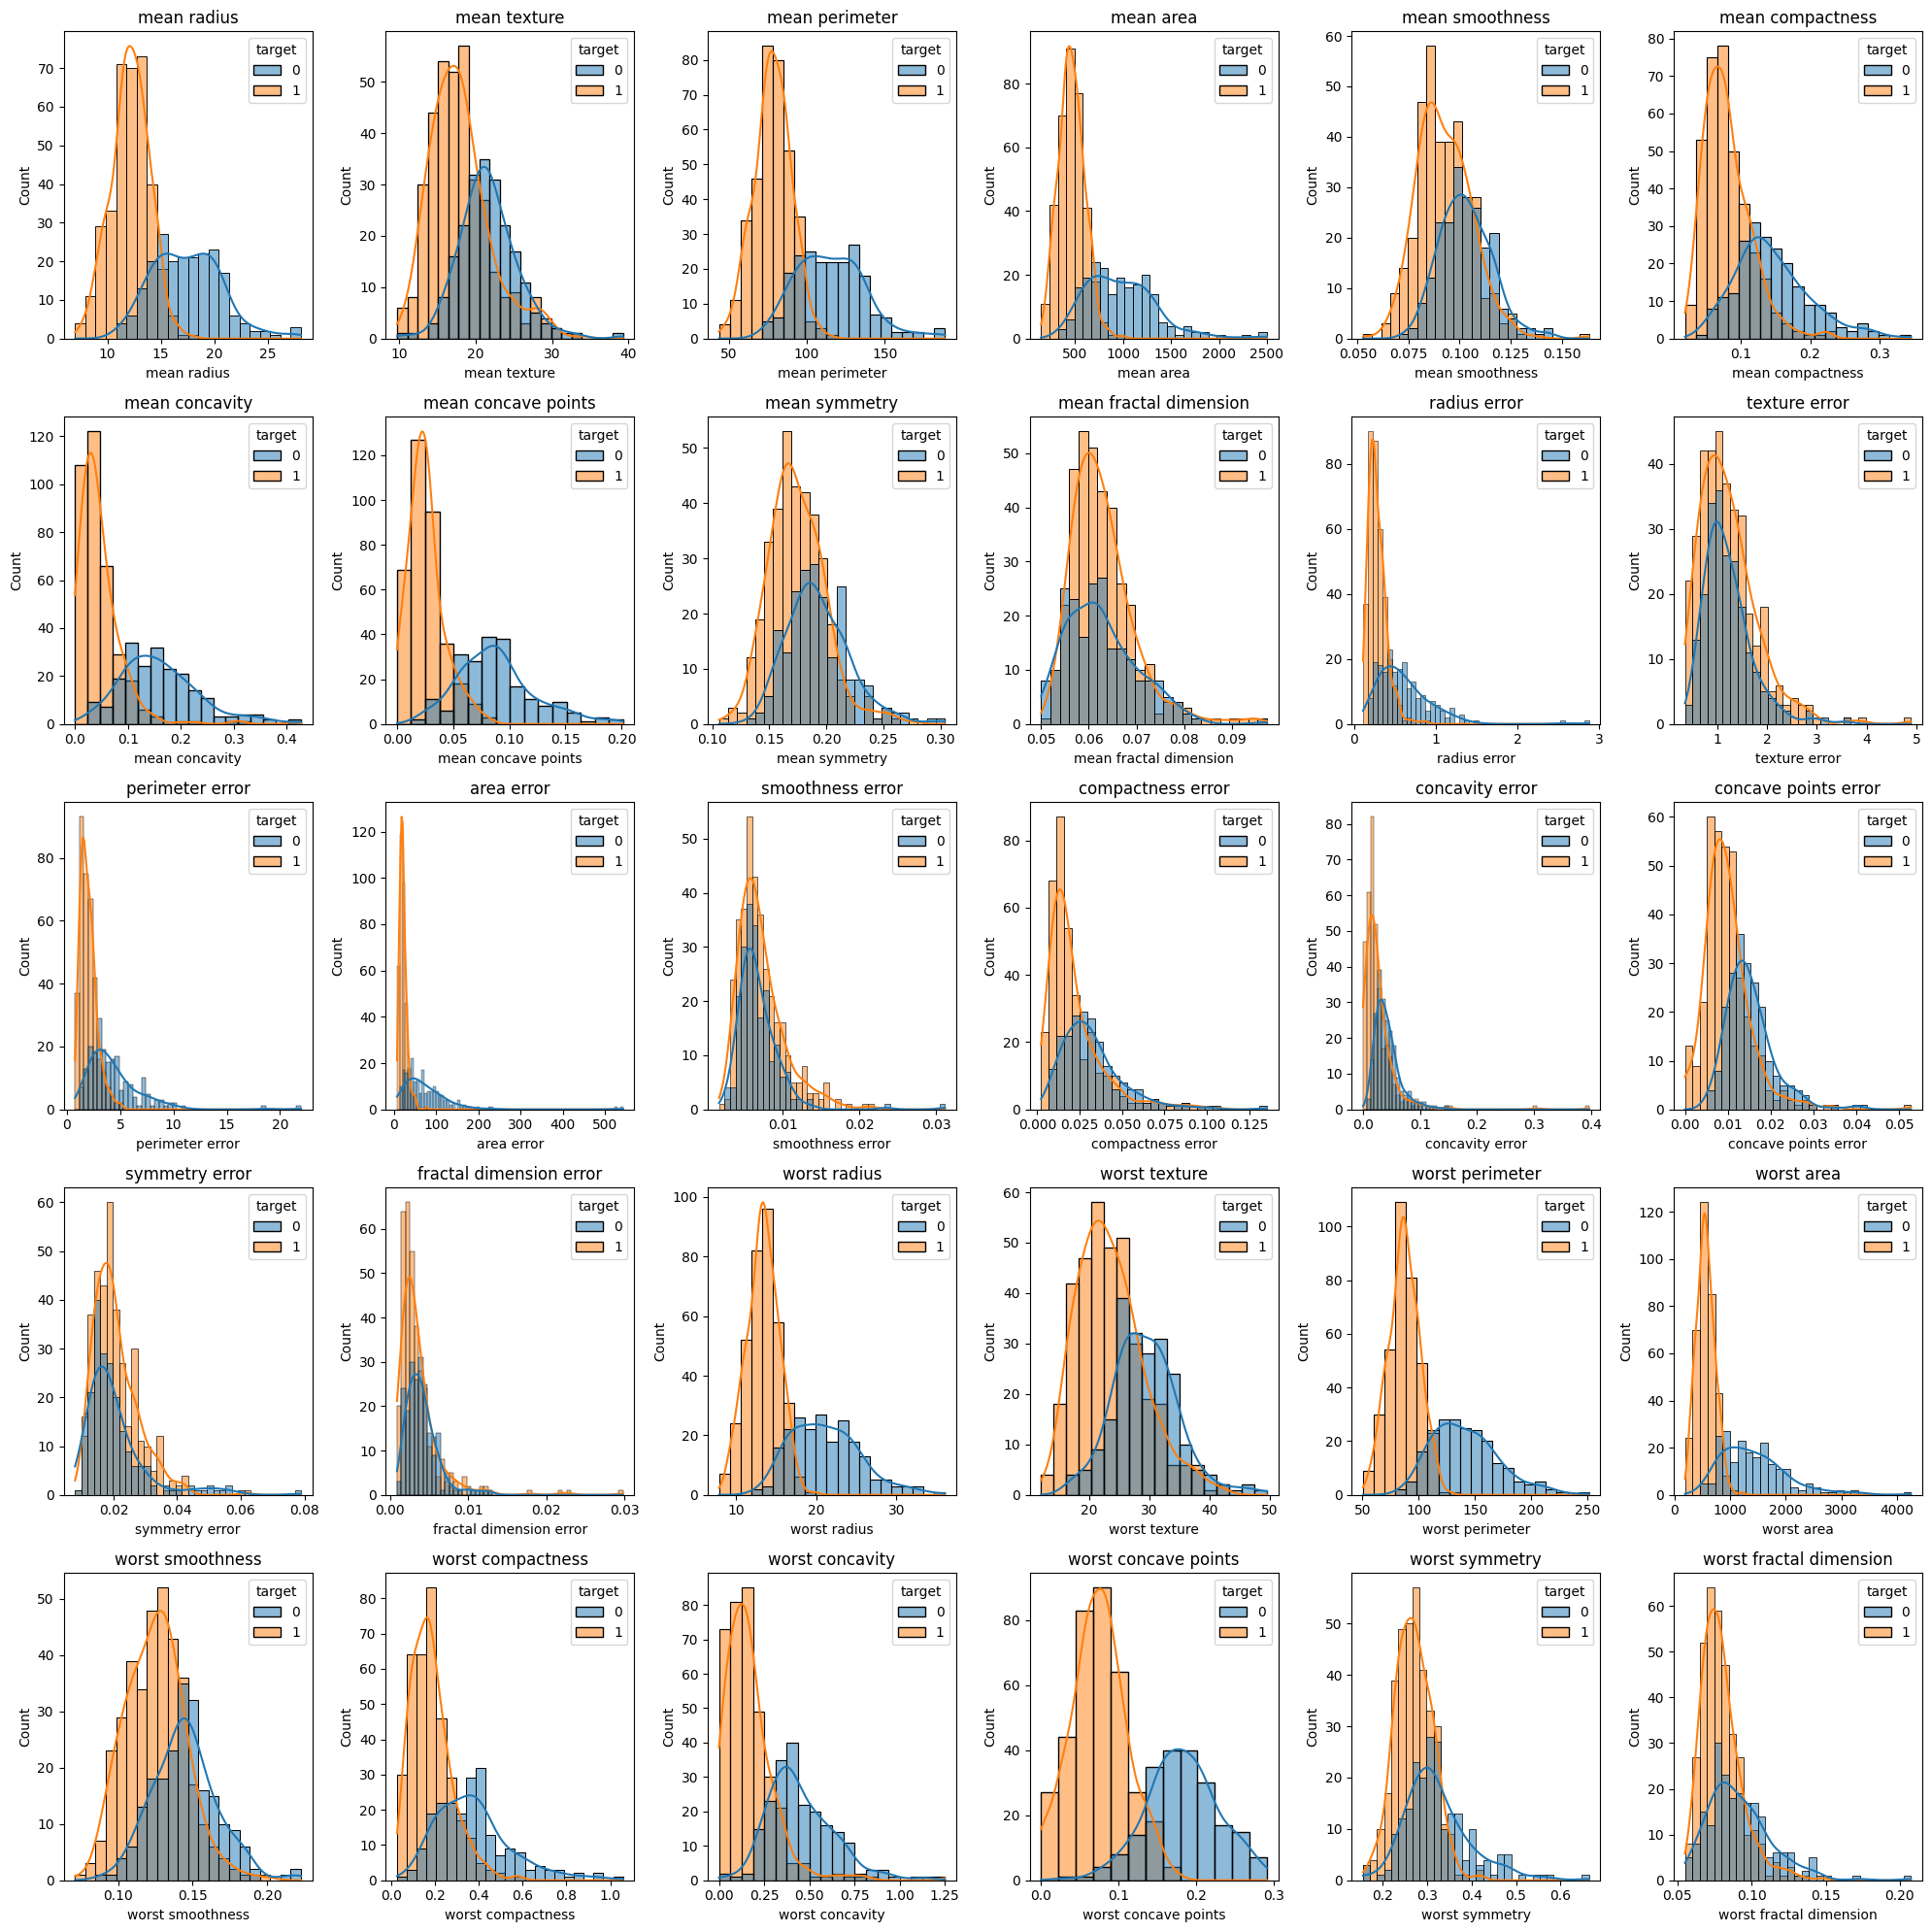
\includegraphics[width=\textwidth]{assets/histograms.png}
        \caption{Histograms for all features labeled by class .}
        \label{fig:histograms_all}
    \end{minipage}
    \hfill
    % Boxplots
    \begin{minipage}{0.49\textwidth}
        \centering
        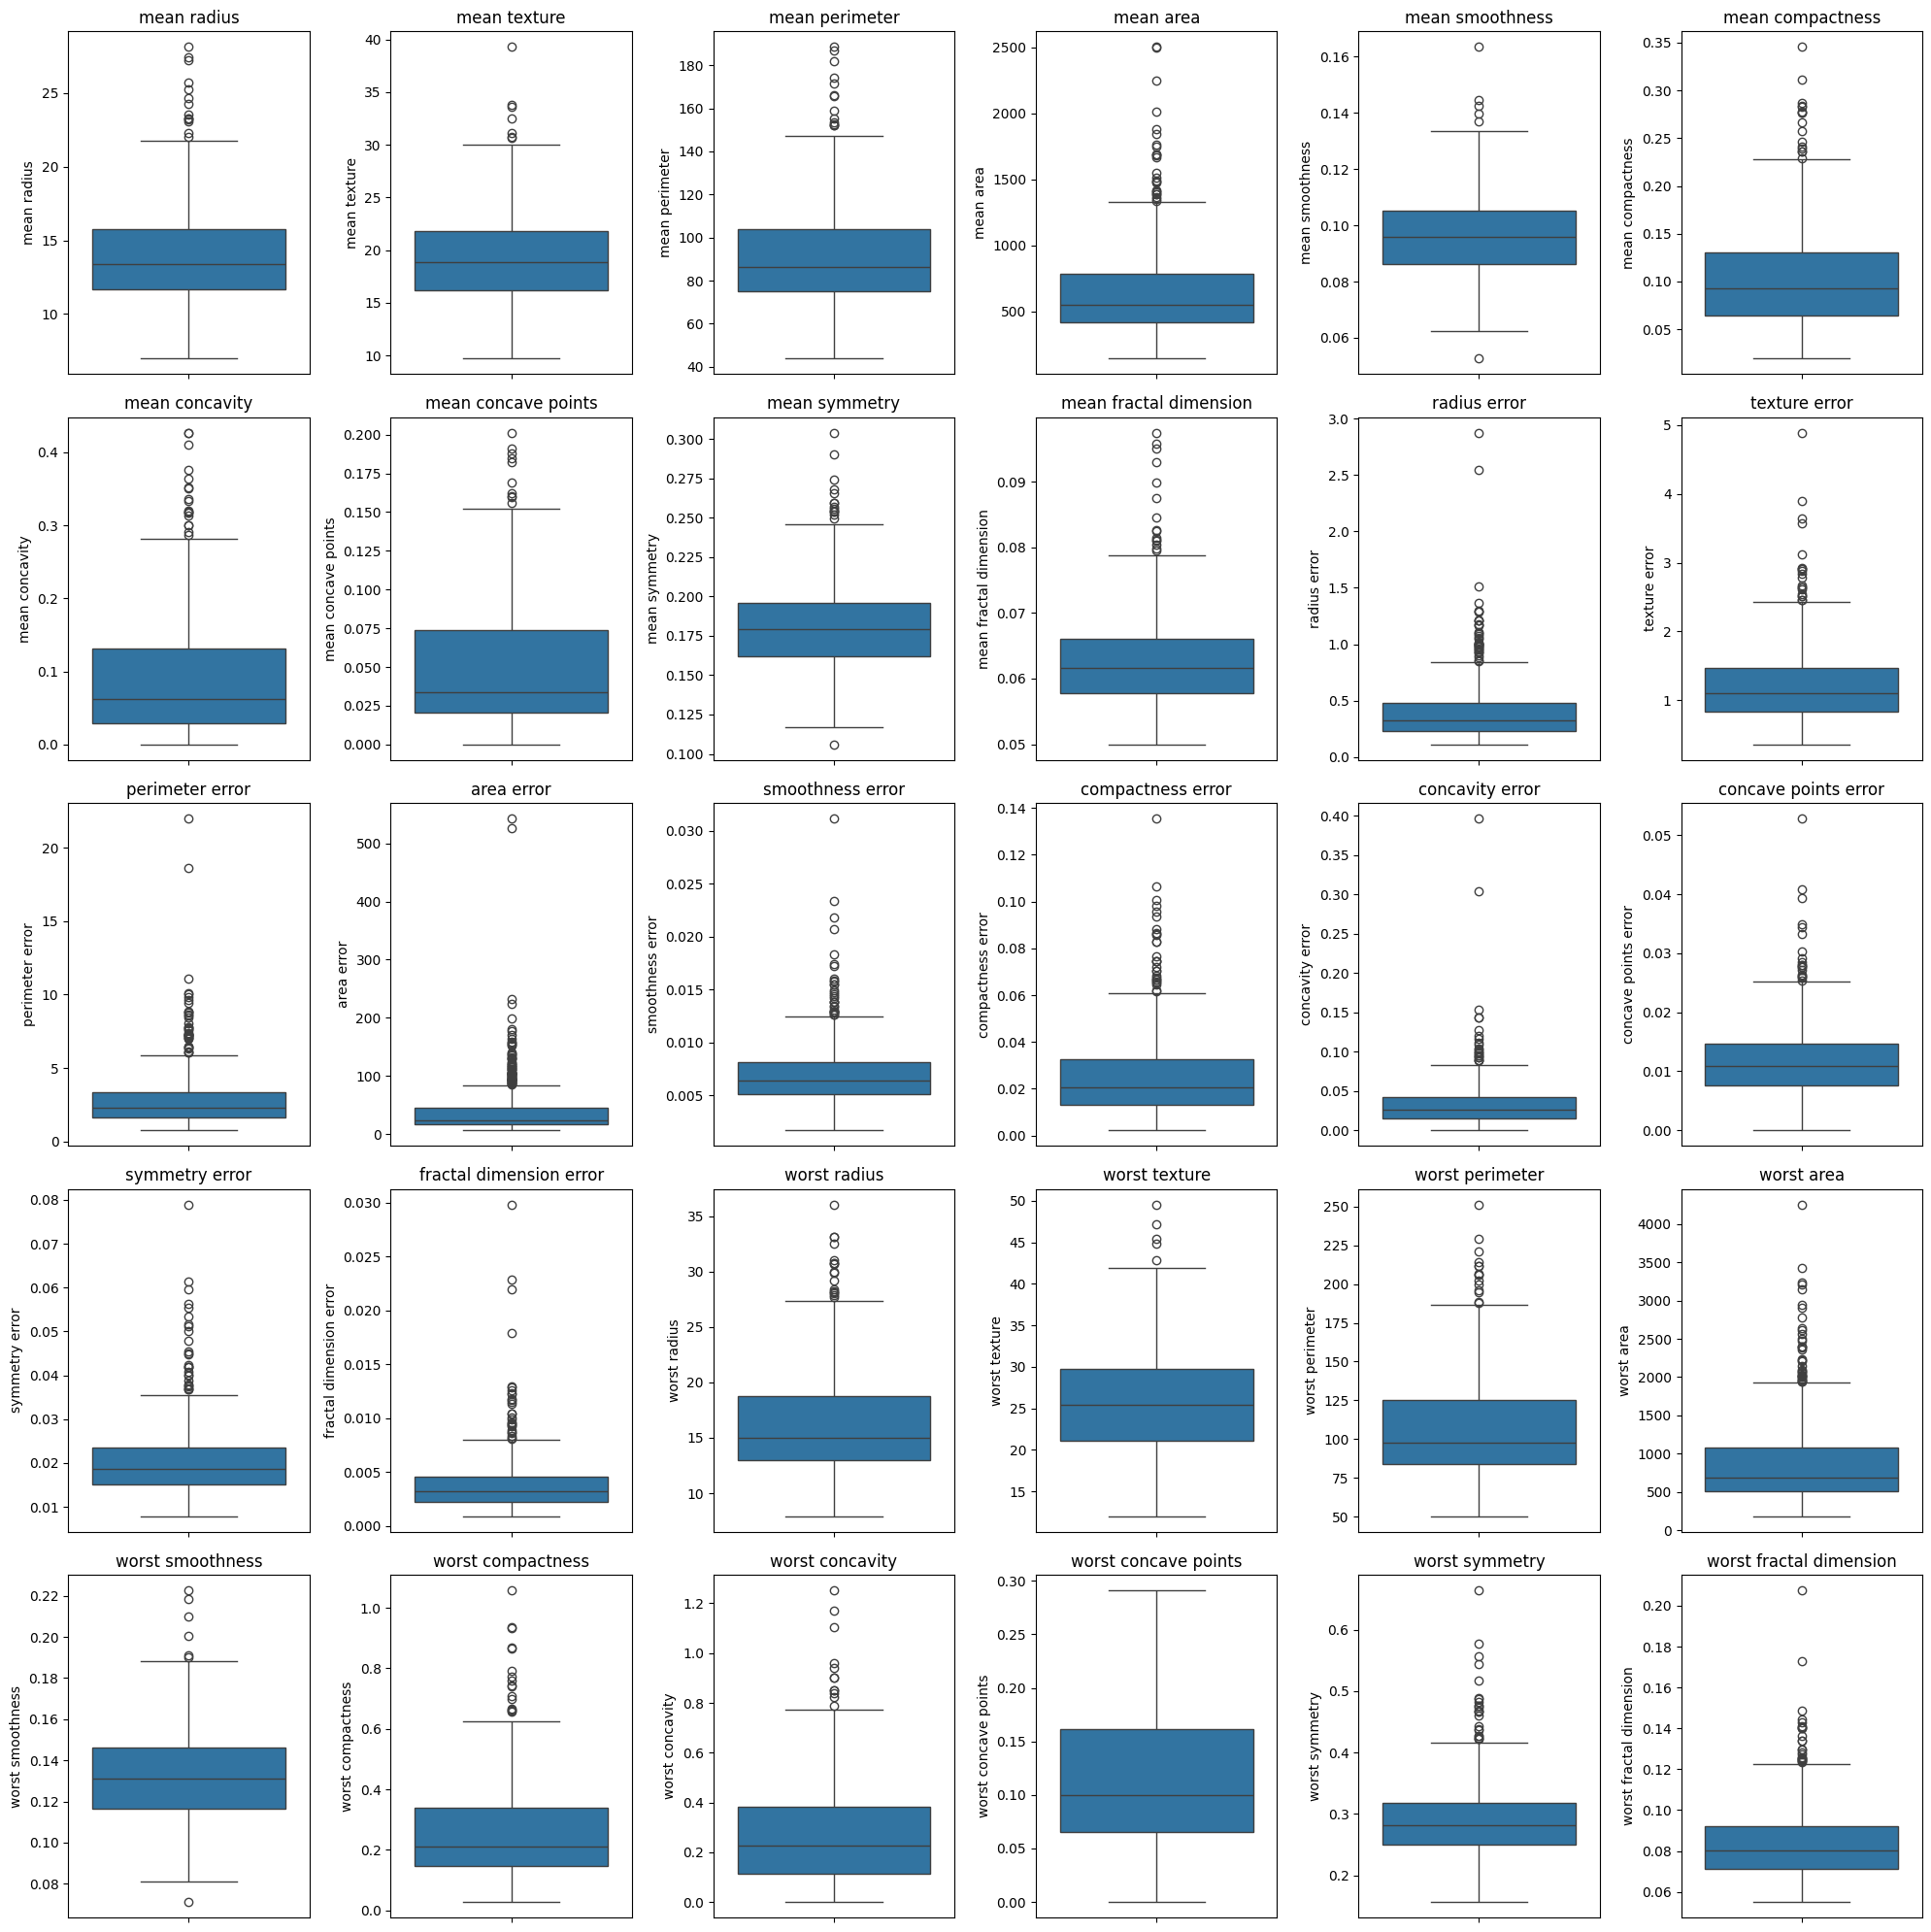
\includegraphics[width=\textwidth]{assets/boxPlots.png}
        \caption{Box plots for all features.}
        \label{fig:boxplots_all}
    \end{minipage}
    
\end{figure}



In summary, the dataset is clean, free of missing values or outliers, and exhibits meaningful feature relationships. These insights provide a solid foundation for training and evaluating machine learning models in subsequent sections. 

The features have been standardized by removing the mean and scaling to unit variance. The dataset was split into training and testing sets with ratio of (75:25)


\section{K-Nearest Neighbors (KNN)}


The K-Nearest Neighbors (KNN) algorithm was implemented and evaluated on the Breast Cancer dataset. The goal was to optimize the model by tuning the distance metrics and the number of neighbors ($k$) using cross-validation.\cite{guo2003knn}

\subsection*{Hyperparameter Tuning}
The following distance metrics were considered for evaluation:
\[
Euclidean, Manhattan, Cosine, Minkowski
\]
Additionally, various values for the number of neighbors were tested:
\[
k = [1, 3, 5, 7, 9, 15]
\]
A grid search was conducted using 5-fold cross-validation, optimizing for classification accuracy. The search space included both the distance metrics and $k$ values. 

\vspace{-10pt} % Reduce vertical space after the figure

\begin{figure}[h!]
    \centering
    % First Subfigure: Varying Distance Metrics
    \begin{subfigure}[b]{0.32\textwidth}
        \centering
        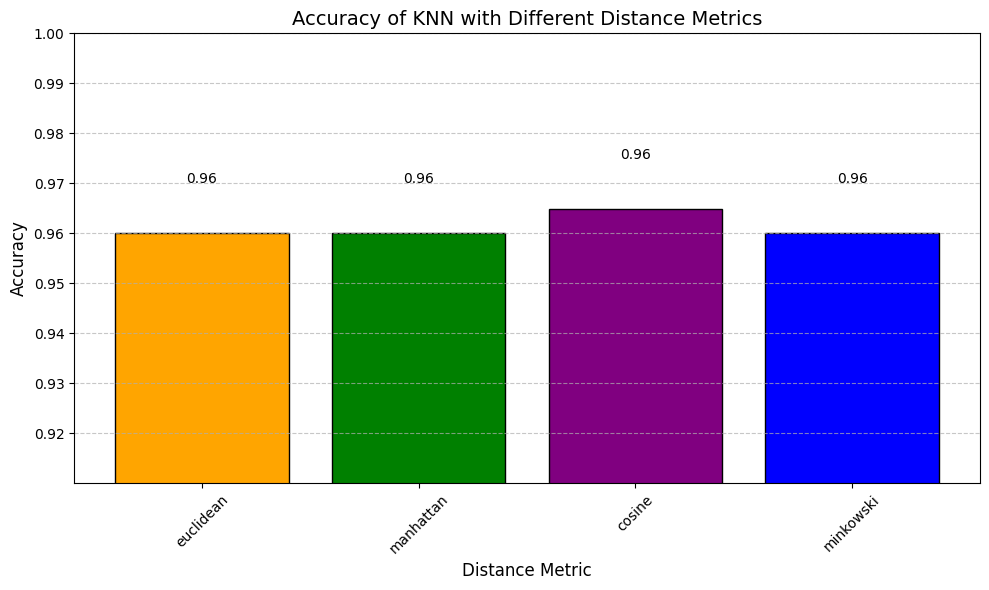
\includegraphics[width=\textwidth]{assets/knn/knn-distance.png}
        \caption{Varying distance metrics.}
        \label{fig:knn_varying_distance}
    \end{subfigure}
    \hfill
    % Second Subfigure: Varying K
    \begin{subfigure}[b]{0.32\textwidth}
        \centering
        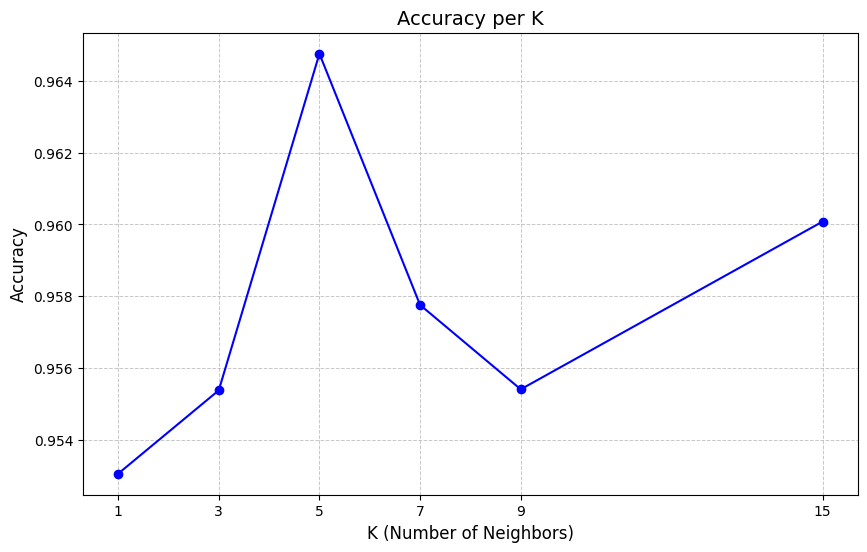
\includegraphics[width=\textwidth]{assets/knn/knn-k.png}
        \caption{Varying $k$ values.}
        \label{fig:knn_varying_k}
    \end{subfigure}
    \hfill
    % Third Subfigure: Combined Effect
    \begin{subfigure}[b]{0.3\textwidth}
        \centering
        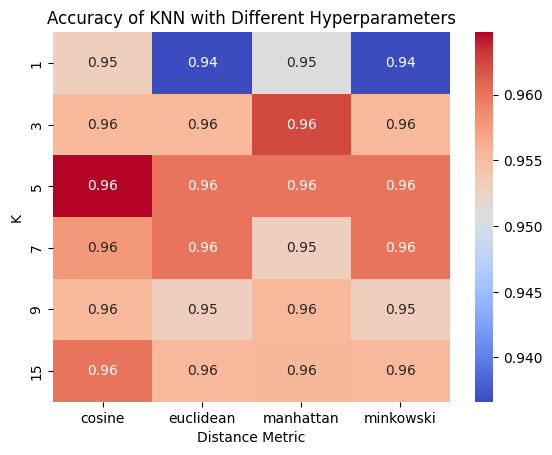
\includegraphics[width=\textwidth]{assets/knn/knn-all.png}
        \caption{Combined.}
        \label{fig:knn_varying_distance_and_k}
    \end{subfigure}

    \caption{KNN performance analysis: (a) varying distance metrics, (b) varying $k$ values, and (c) combined effect of distance metrics and $k$.}
    \label{fig:knn_subfigures}
\end{figure}







\subsection*{Training and Evaluation}

Using the best hyperparameters identified from grid search, the KNN model was trained with: \textbf{Number of Neighbors:} 5, \textbf{Distance Metric:} Cosine. The model was then tested on the unseen test set.


\subsection*{Results}

\textbf{Classification Report:}
\begin{verbatim}
              precision    recall  f1-score   support
           0       0.93      0.96      0.95        54
           1       0.98      0.96      0.97        89
    accuracy                           0.96       143
\end{verbatim}

\textbf{Confusion Matrix:} Figure~\ref{fig:confusion_matrix_knn} shows the confusion matrix for the KNN classifier.

\textbf{ROC Curve and AUC Score:} The ROC curve is shown in Figure~\ref{fig:roc_curve_knn}, with the Area Under the Curve (AUC) score of 0.985, indicating strong model performance.


\begin{figure}[h!]
    \centering
    % Confusion Matrix
    \begin{subfigure}[b]{0.4\textwidth}
        \centering
        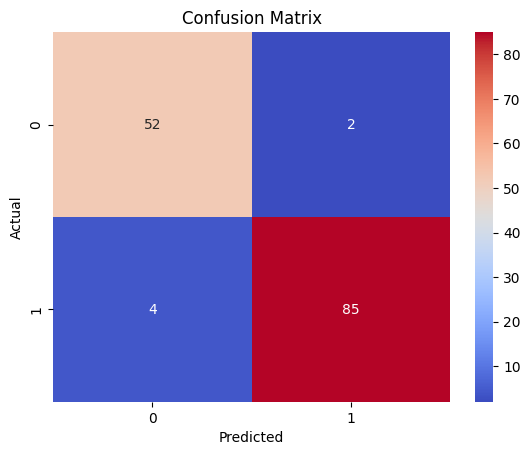
\includegraphics[width=\textwidth]{assets/knn/knn-cm.png}
        \caption{Confusion matrix for the KNN model.}
        \label{fig:confusion_matrix_knn}
    \end{subfigure}
    \hfill
    \begin{subfigure}[b]{0.4\textwidth}
        \centering
        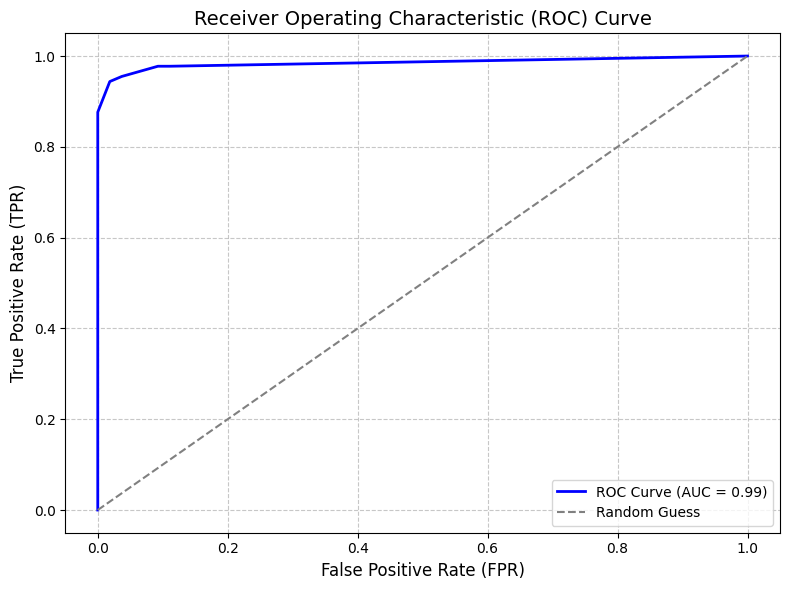
\includegraphics[width=\textwidth]{assets/knn/knn-roc.png}
        \caption{ROC Curve for the KNN model.}
        \label{fig:roc_curve_knn}
    \end{subfigure}
    \vspace{-10pt} % Reduce vertical space after the figure
    \caption{Performance evaluation of the KNN model: (a) Confusion matrix and (b) ROC curve.}
    \label{fig:knn_side_by_side}
\end{figure}


\vspace{-15pt} % Reduce vertical space after the figure
The KNN model performed well on the Breast Cancer dataset, achieving high accuracy and an AUC score of 0.985. The Cosine distance metric and $k=5$ were found to be optimal hyperparameters. This indicates that the model effectively captured the underlying patterns in the data.

\section{Logistic Regression}
Logistic Regression was evaluated on the Breast Cancer dataset with a focus on tuning the regularization technique and strength. Regularization helps in preventing overfitting by penalizing large coefficients, with two options being considered:

\vspace{-0.35cm}

\textbf{L1 (Lasso):} Adds an absolute magnitude penalty on coefficients, potentially reducing some to zero (feature selection).  \textbf{L2 (Ridge):} Adds a squared magnitude penalty on coefficients, shrinking them towards zero but never eliminating features. 

\vspace{-0.35cm}

The regularization strength $C$ is inversely proportional to the regularization applied. A smaller $C$ imposes stronger regularization, shrinking coefficients and reducing model complexity, while a larger  $C$ reduces regularization, allowing the model to fit the training data more closely.\cite{qin20191}

\subsection*{Hyperparameter Tuning}

A grid search was conducted using 5-fold cross-validation to evaluate the following hyperparameters: \textbf{Penalties:} L1, L2, \textbf{Regularization Strength  C:} [0.001, 0.01, 0.1, 1, 10, 100] 

\setlength{\textfloatsep}{5pt} % Reduce space after the figure
\begin{figure}[H]
\centering 
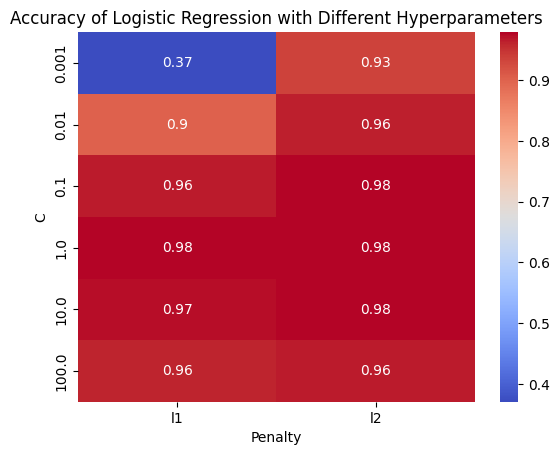
\includegraphics[width=0.4\textwidth]{assets/lr/lr-param.png} \caption{Accuracy of Logistic Regression with different hyperparameters.} \label{fig:logreg_heatmap} \end{figure}
\vspace{-20pt} % Reduce vertical space after the figure
\subsection*{Training and Evaluation}

Using the best hyperparameters identified from grid search, the logistic regression model was trained with: \textbf{Penalty:} L2, \textbf{C:} 1. The model was then tested on the unseen test set.


\subsection*{Results}
\textbf{Classification Report:}
\begin{verbatim}
              precision    recall  f1-score   support
           0       0.96      0.96      0.96        54
           1       0.98      0.98      0.98        89
    accuracy                           0.97       143
\end{verbatim}
\vspace{-10pt} % Reduce vertical space after the figure

\textbf{Confusion Matrix:} Figure~\ref{fig:confusion_matrix_lr} shows the confusion matrix for the logistic regression classifier.
\textbf{ROC Curve and AUC Score:} The ROC curve is shown in Figure~\ref{fig:roc_curve_lr}, with the Area Under the Curve (AUC) score of 0.997, indicating strong model performance.
\begin{figure}[H]
    \centering
    % Confusion Matrix
    \begin{subfigure}[b]{0.4\textwidth}
        \centering
        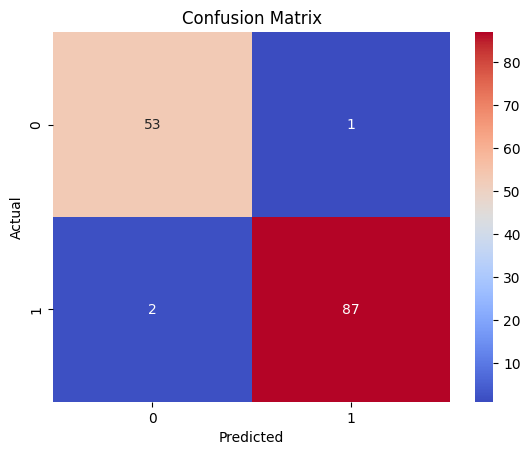
\includegraphics[width=\textwidth]{assets/lr/lr-cm.png}
        \caption{Confusion matrix for the model.}
        \label{fig:confusion_matrix_lr}
    \end{subfigure}
    \hfill
    % ROC Curve
    \begin{subfigure}[b]{0.4\textwidth}
        \centering
        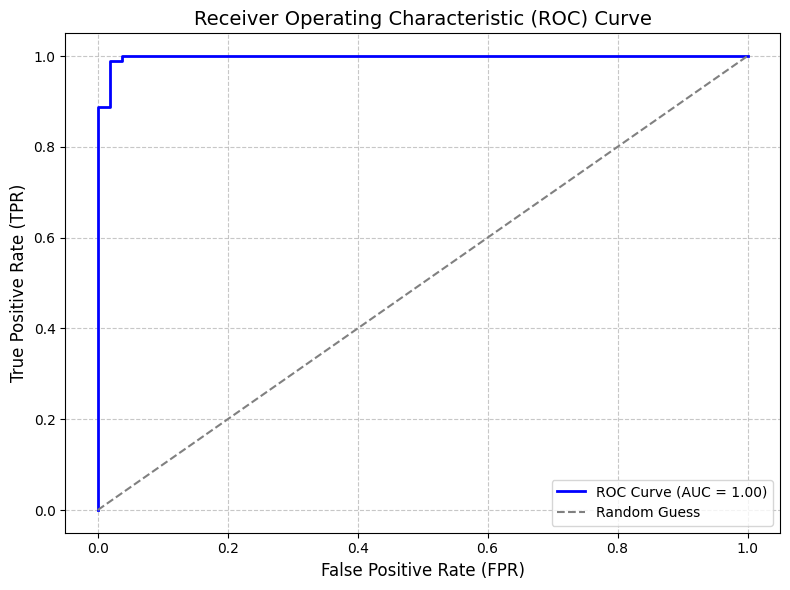
\includegraphics[width=\textwidth]{assets/lr/lr-roc.png}
        \caption{ROC Curve for the model.}
        \label{fig:roc_curve_lr}
    \end{subfigure}
    \caption{Performance evaluation of the logistic regression model: (a) Confusion matrix and (b) ROC curve.}
    \label{fig:lr_side_by_side}
\end{figure}
\vspace{-15pt} % Reduce vertical space after the figure

\vspace{-0.35cm}

The results show that \textbf{Logistic Regression} did a bit better than \textbf{KNN}, with \textbf{97\% accuracy} and \textbf{0.997 ROC-AUC}, while knn got \textbf{96\% accuracy} and \textbf{0.985 ROC-AUC}. KNN worked best using \(k=5\) and Cosine distance, while Logistic Regression used L2 regularization and \(C=1\).




\section{Support Vector Machines (SVM)}


Support Vector Machines (SVM) were implemented to classify the Breast Cancer dataset. We experimented with multiple kernels: \textbf{linear}, \textbf{polynomial (poly)}, \textbf{radial basis function (RBF)}, and \textbf{sigmoid}. A grid search with 5-fold cross-validation was conducted to tune the regularization parameter \(C\) values: [0.01, 0.1, 0.2, 1, 10, 100].\cite{hearst1998support}

\subsection*{Hyperparameter Tuning}

The performance of the kernels with different \(C\) values was evaluated and visualized using a heatmap. Figure~\ref{fig:svm_heatmap} shows the accuracy scores for each combination of kernel and \(C\).  

\begin{figure}[H]
    \centering
    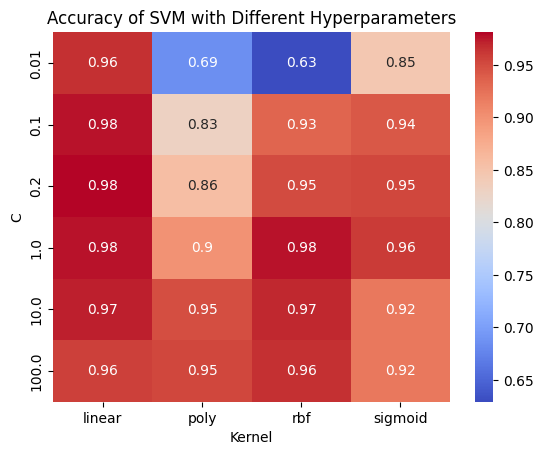
\includegraphics[width=0.4\textwidth]{assets/svm/svm-param.png}
    \caption{Accuracy of SVM with different kernels and \(C\) values.}
    \label{fig:svm_heatmap}
\end{figure}
\vspace{-0.5cm}
\subsection*{Training and Evaluation}

Using the best parameters identified from grid search (\textbf{Kernel: Linear, \(C=0.2\)}), the SVM model was trained and evaluated on the test set.

\begin{verbatim}
              precision    recall  f1-score   support
           0       0.96      0.96      0.96        54
           1       0.98      0.98      0.98        89
    accuracy                           0.97       143
\end{verbatim}

\textbf{Confusion Matrix and ROC Curve:} Figure~\ref{fig:svm_cm_roc} presents the confusion matrix and ROC curve for the SVM model.

\begin{figure}[H]
    \centering
    \begin{subfigure}[b]{0.4\textwidth}
        \centering
        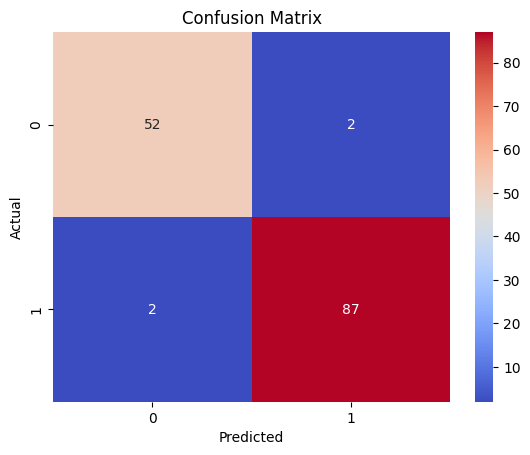
\includegraphics[width=\textwidth]{assets/svm/svm-cm.png}
        \caption{Confusion Matrix}
        \label{fig:svm_cm}
    \end{subfigure}
    \hfill
    \begin{subfigure}[b]{0.4\textwidth}
        \centering
        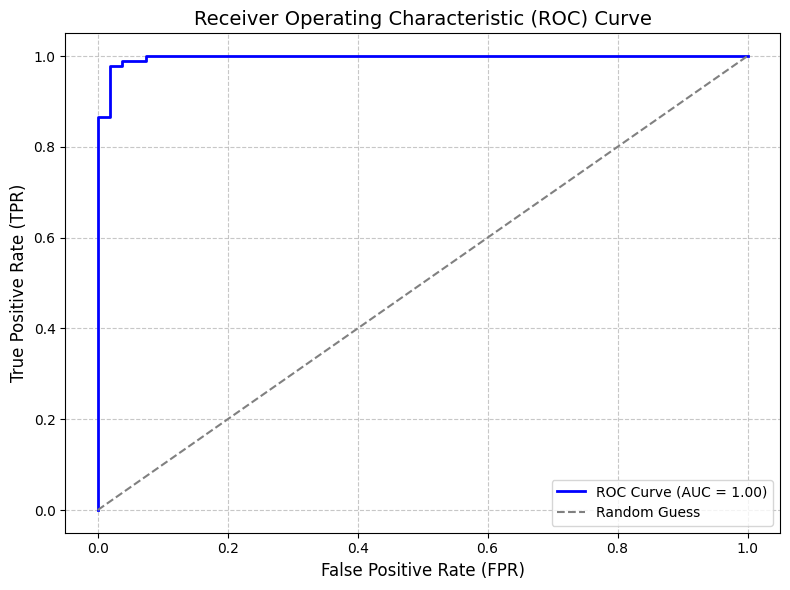
\includegraphics[width=\textwidth]{assets/svm/svm-roc.png}
        \caption{ROC Curve (AUC = 0.997 )}
        \label{fig:svm_roc}
    \end{subfigure}
    \caption{Performance evaluation of the SVM model.}
    \label{fig:svm_cm_roc}
\end{figure}

\subsection*{Impact of Kernels}

The choice of kernel significantly impacted the performance of the SVM model. The \textbf{linear kernel} provided the best results with an accuracy of 97\%, while the \textbf{RBF kernel} performed similarly. Polynomial and sigmoid kernels performed worse, likely due to overfitting or a poor fit to the dataset structure. The linear kernel’s simplicity and effectiveness made it the optimal choice for this dataset.



The SVM model, using a linear kernel with \(C=0.2\), achieved high performance with an accuracy of 97\% and an AUC score of 0.997, making it a robust choice for this classification task.



\section{Ensemble Methods}
Ensemble methods combine an ensemble (group) of learners (classifiers) together into a stronger classifier. It is subdivided into two categories: Boosting and Bagging.
\par
Boosting methods typically use weak learners, where each subsequent learner is trained on the same dataset with adjusted sample weight depending on the mistakes the previous estimators make. AdaBoost is one of the boosting methods that uses decision stumps as learners.
\par
Bagging methods typically use strong learners, where each learner is trained on a bootstrap sample of the dataset. Random forest is one of the bagging methods that uses decision trees as learners.
\subsection{Boosting \textemdash AdaBoost}
\textbf{AdaBoost} was implemented to classify the Breast Cancer dataset. To find the best hyperparameters, we experimented with \textbf{number of estimators}: [100, 300, 500, 700, 900, 1100, 1300, 1500, 1700, 1900], and \textbf{learning rate}: [0.01, 0.05, 0.1, 0.5, 1.0, 1.4, 1.5, 1.6, 2, 3]. A grid search with 5-fold cross-validation was conducted to identify the best hyperparameters.\cite{hastie2009multi}
\subsubsection*{Hyperparameter Tuning}
The performance of the each pair of hyperparameters was evaluated and visualized. Figure~\ref{fig:ada_param} shows the accuracy scores for each pair of \textbf{learning rate} and \textbf{number of estimators}
\begin{figure}[H]
    \centering
    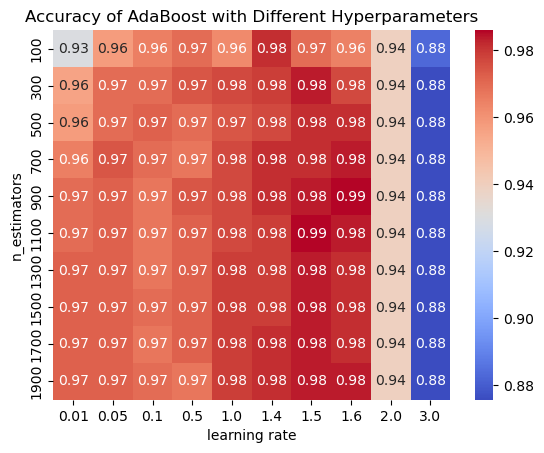
\includegraphics[width=0.5\linewidth]{assets/ada/ada-param.png}
    \caption{Accuracy of AdaBoost with different number of estimators and learning rate.}
    \label{fig:ada_param}
\end{figure}
\subsubsection*{Training and Evaluation}
Using the best parameters from the grid search (\textbf{number of estimators}: 1100, \textbf{learning rate}: 1.5, the AdaBoost model was trained and evaluated on the test set.
\begin{verbatim}
              precision    recall  f1-score   support
           0       0.95      0.98      0.96        54
           1       0.99      0.97      0.98        89
    accuracy                           0.97       143
\end{verbatim}
\textbf{Confusion Matrix and ROC Curve:} Figure~\ref{fig:ada_cm_roc} represents the confusion matrix and ROC curve of the AdaBoost model.
\begin{figure}[H]
    \centering
    \begin{subfigure}[b]{0.4\textwidth}
        \centering
        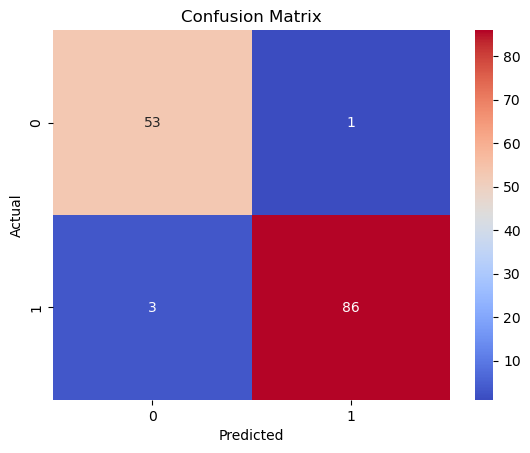
\includegraphics[width=\textwidth]{assets/ada/ada-cm.png}
        \caption{Confusion Matrix}
        \label{fig:ada_cm}
    \end{subfigure}
    \hfill
    \begin{subfigure}[b]{0.4\textwidth}
        \centering
        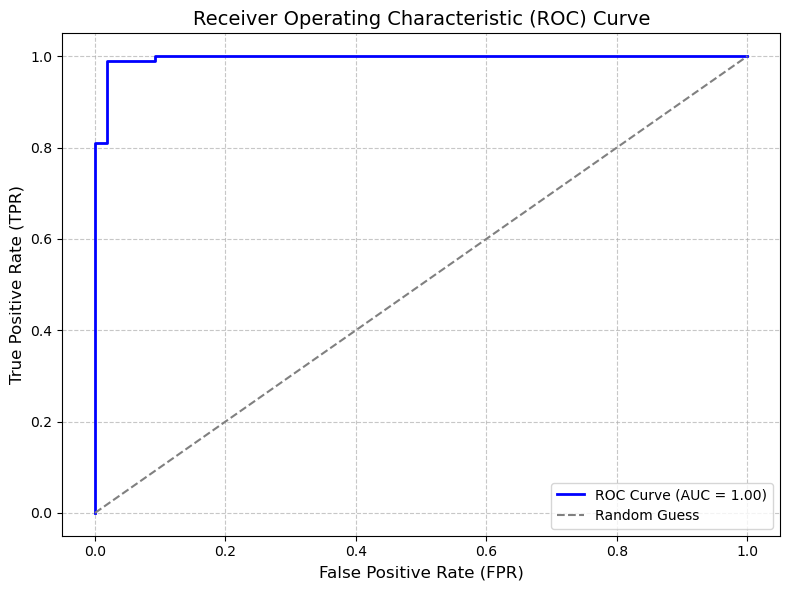
\includegraphics[width=\textwidth]{assets/ada/ada-roc.png}
        \caption{ROC Curve (AUC = 0.995)}
        \label{fig:ada_roc}
    \end{subfigure}
    \caption{Performance evaluation of the AdaBoost Model.}
    \label{fig:ada_cm_roc}
\end{figure}

\vspace{-0.8cm}

\subsubsection*{Impact of Learning Rate}
The \textbf{learning rate} controls how much the weights of misclassified samples increase after each estimator. A very low learning rate slows learning as reweighing is minimal, while a high learning rate overly emphasizes misclassified samples, effectively \textbf{ignoring} correctly classified ones.
\par
A low learning rate with enough estimators yields decent results, but a high learning rate can drastically harm accuracy.
\subsubsection*{Impact of N estimators}
Increasing the \textbf{number of estimators} decreases the \textbf{bias} and increases the \textbf{variance}. As the dataset is relatively not noisy, and we are using decision stomps as estimator in AdaBoost, setting the number of estimators relatively high doesn't lead to over fitting. Obviously, the increasing number of estimators impacts computational efficiency.
\subsection{Bagging \textemdash Random Forest}
\textbf{Random Forest (RF)} was implemented to classify the Breast Cancer dataset. To find the best hyperparameters, we experimented with \textbf{number of estimators}: [50, 80, 100,200, 300, 500, 700, 900, 1100, 1300, 1500, 1700, 1900], \textbf{max features}: [log2, sqrt],  and \textbf{max depth}: [1, 5, 10, 30, inf. A grid search with 5-fold cross-validation was conducted to identify the best hyperparameters.\cite{breiman2001random}
\subsubsection*{Hyperparameter Tuning}
The performance of the each combination of hyperparameters was evaluated and visualized. Figure~\ref{fig:rf_param} shows the accuracy scores for different combination of hyperparameters.
\begin{figure}[H]
    \centering
    \begin{subfigure}[b]{0.4\textwidth}
        \centering
        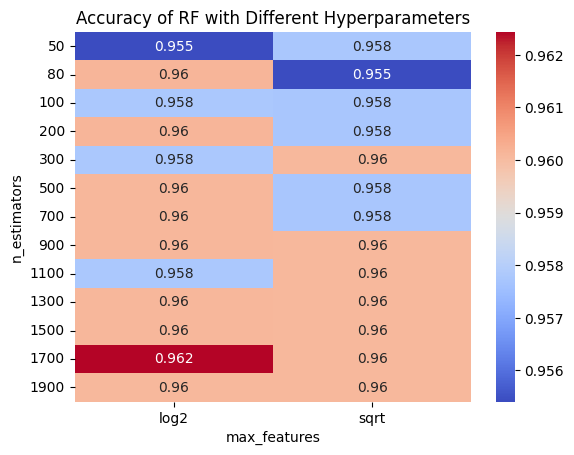
\includegraphics[width=\textwidth]{assets/rf/rf-param1.png}
        \caption{Best number of estimators and maximum features to consider when finding the best split.}
        \label{fig:rf_param1}
    \end{subfigure}
    \hfill
    \begin{subfigure}[b]{0.4\textwidth}
        \centering
        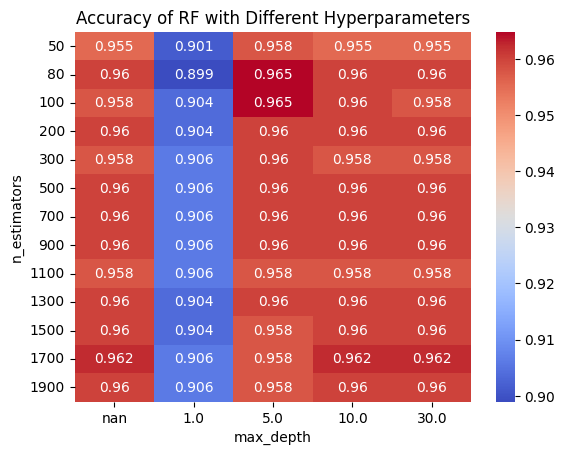
\includegraphics[width=\textwidth]{assets/rf/rf-param2.png}
        \caption{Best number of estimators and maximum depth.}
        \label{fig:rf_param2}
    \end{subfigure}
    \caption{Accuracy of Random Forest with different hyperparameters.}
    \label{fig:rf_param}
\end{figure}
\subsubsection*{Training and Evaluation}
Using the best parameters from the grid search (\textbf{number of estimators}: 80, \textbf{max depth}: 5, \textbf{max features}: log2, the RF model was trained and evaluated on the test set.
\begin{verbatim}
 precision    recall  f1-score   support

   0       0.96      0.94      0.95        54
   1       0.97      0.98      0.97        89

 accuracy                      0.97       143
\end{verbatim}
\textbf{Confusion Matrix and ROC Curve:} Figure~\ref{fig:rf_cm_roc} represents the confusion matrix and ROC curve of the RF model.
\begin{figure}[H]
    \centering
    \begin{subfigure}[b]{0.4\textwidth}
        \centering
        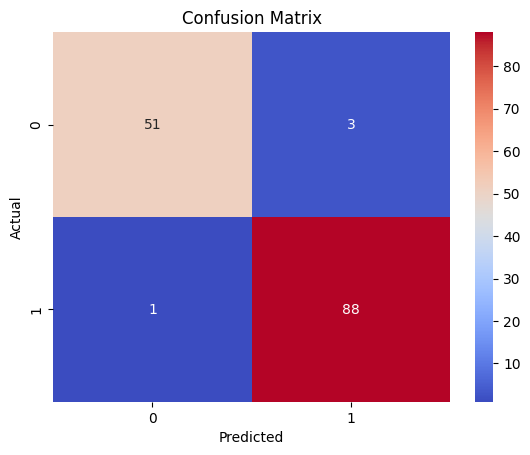
\includegraphics[width=\textwidth]{assets/rf/rf-cm.png}
        \caption{Confusion Matrix}
        \label{fig:rf_cm}
    \end{subfigure}
    \hfill
    \begin{subfigure}[b]{0.4\textwidth}
        \centering
        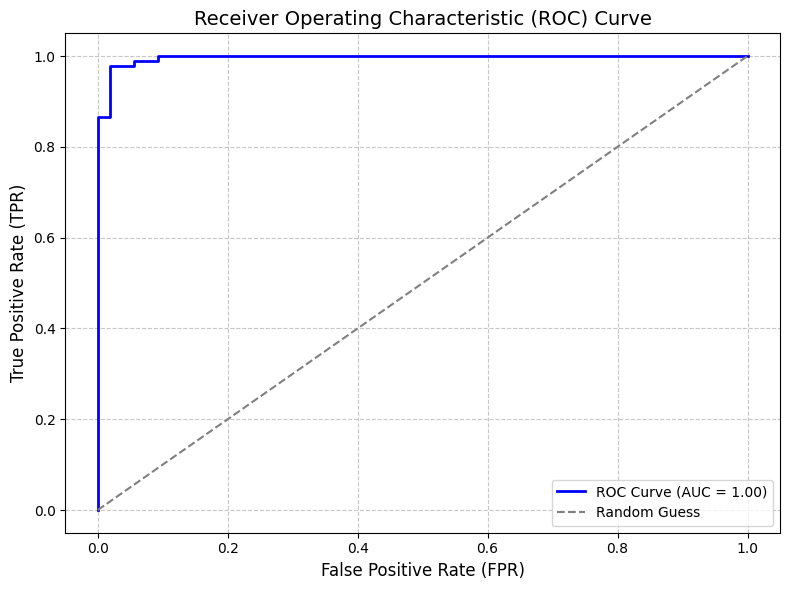
\includegraphics[width=\textwidth]{assets/rf/rf-roc.png}
        \caption{ROC Curve (AUC = 0.996)}
        \label{fig:rf_roc}
    \end{subfigure}
    \caption{Performance evaluation of the Random Forest Model.}
    \label{fig:rf_cm_roc}
\end{figure}

\vspace{-0.8cm}

\subsubsection*{Impact Max Depth}
As each tree in RF learns on a bootstrap sample, it is very hard to overfit the data with a high number of estimators as the variation between datasets is high. However, each decision tree may start over fitting its own bootstrap sample interpreting noise and randomness as features. To limit this behavior, the maximum depth of each tree is bounded by this parameter.

\section{Conclusion}
Based on the high accuracy achieved with most methods the dataset is of very high quality with very few outliers. As a medical decision is made based on the classification result, it's important to decide whether the test is suggestive (higher recall is preferable), or confirmatory (higher precision is preferable). It may also be important to be able to explain the results to doctors, which may not be possible for some models (eg. explaining an AdaBoost model with a 1100 estimators).
\par
Based on table~\ref{tab:model_metrics}, \textbf{Logistic} regression (LR) with L2 regularization parameter $C = 1$, provides the best performance across \textbf{all} metrics. Despite high dimensionality of the dataset, the linear boundary generated by LR is simple enough to explain it to a doctor. The default threshold (0.5) is showing great results, but it could be further adjusted to favor false negatives or false positives (see figure~\ref{fig:roc_curve_lr}).

\begin{table}[h!]
\centering
\begin{tabular}{|l|c|c|c|c|c|}
\hline
\textbf{Metric}   & \textbf{KNN} & \textbf{Logistic} & \textbf{SVM} & \textbf{RF} & \textbf{AdaBoost} \\ \hline
Precision         & 0.98         & 0.99              & 0.98         & 0.97        & 0.99              \\ \hline
Recall            & 0.96         & 0.98              & 0.98         & 0.98        & 0.97              \\ \hline
F1-Score          & 0.97         & 0.98              & 0.98         & 0.97        & 0.98              \\ \hline
Accuracy          & 0.96         & 0.98              & 0.97         & 0.97        & 0.97              \\ \hline
AUC               & 0.985        & 0.997             & 0.996        & 0.996       & 0.995             \\ \hline
\end{tabular}
\caption{Performance metrics for all tested models.}
\label{tab:model_metrics}
\end{table}
\printbibliography
\begin{appendices}
\section{Contributions}
\begin{itemize}
    \item \textbf{Mohammed}: Performed Exploratory Data Analysis (EDA), implemented KNN, Logistic Regression, and SVM, and wrote the corresponding sections.
    \item \textbf{Karim}: Handled data preprocessing, implemented Random Forest and AdaBoost, and wrote the corresponding sections, along with the conclusion.
\end{itemize}
\end{appendices}
\end{document}



 